To study the statistical structure of the CMB signal, the cross power spectrum of the sky map is computed. An unbiased estimator is given by [reference Efst?]:

$ insert Cl formula,$
where $a_lm$ corresponds to the Fourier coefficients of the sky's spherical harmonics decomposition:
$ insert alm formula $ 

\vspace{0.2em}
\begin{figure}
	\begin{minipage}{.94\textwidth}
		\centering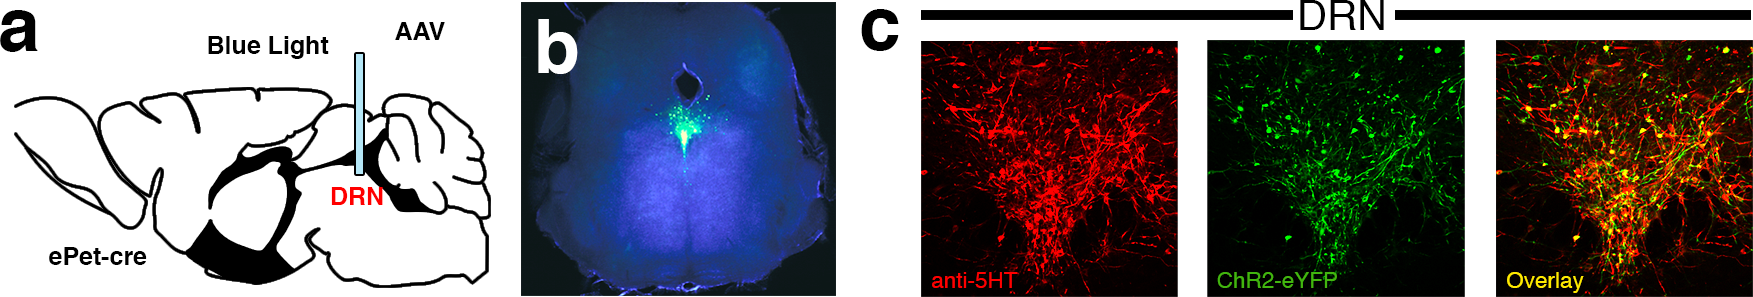
\includegraphics[width=\textwidth]{img/og.png}
		\caption{\textbf{(a)}  Aliquam semper facilisis dui, et gravida libero}
	\end{minipage}
\end{figure}
\vspace{0.4em}
Nullam pulvinar nulla quis felis posuere condimentum. Fusce purus nunc, efficitur nec varius quis, lacinia et lorem. Etiam non sem felis. Etiam imperdiet semper arcu, sodales facilisis dui volutpat quis. Quisque rutrum varius risus, a posuere mi volutpat quis. Aenean ac eros nec neque lacinia luctus ac at erat. Donec ut nisi eget nulla dapibus faucibus. Ut dapibus est non condimentum laoreet. 
